\section {Вычисление асимптотических результатов}
Имитационное моделирование позволяет нам получать большое количество информации о работе системы, и во многих задачах оно используется для определения области применимости асимптотических результатов. В зависимости от задачи они могут быть получены и вычисляться легко, но в других случаях они могут быть представлены в виде характеристической функции, а для анализа проводится поточечное сравнение распределений вероятности исследуемой характеристики системы. Такая функция может содержать трудно поддающиеся вычислению элементы, среди которых находятся интегралы, матричные экспоненты и др., поскольку получена она была при помощи математического аппарата без первостепенной задачи оптимизации ее вычисления. И на этапе, когда требуется получить значения такой функции, процесс оказывается длительным и трудоемким, так как переход от характеристической функции к распределению вероятностей производится при помощи обратного преобразования Фурье, использующего интегрирование. В ситуации, когда характеристическая функция имеет два, три и более аргументов, вычислительная сложность возрастает во много раз в виду вложенных интегралов. К проблеме трудоемкости также добавляется надобность производить большое количество вычислений, например, для пятисот запусков имитационной модели, результатом которых будет являться двумерное распределение вероятностей размерностью 10 на 10 точек, потребуется 500 раз вычислить то же самое распределение посредством аналитических формул.

В данном разделе предлагается использовать теорию Фурье-анализа сигналов для обращения характеристических функций дискретных распределений. Идея заключается в применении принципов теоремы Котельникова \cite{ястребов2012дискретизация,kuznecov2008} для дискретизации характеристических функций и применения дискретного преобразования Фурье, которое вместо интегрирования использует суммирование и умножение, что гораздо эффективнее. В рамках разрабатываемого программного комплекса этот подход также применяется для обращения характеристической функции и упрощения вычислений, связанных с этим процессов. Данное решение может быть использовано как для анализа систем массового обслуживания, так и в других разделах теории вероятностей, где требуются множественные вычисления.

Как известно, любая случайная величина может быть однозначно определена функцией распределения вероятностей или характеристической функцией \cite{gnedenko2010}. При этом характеристическая функция может быть определена для любой случайной величины (дискретной или непрерывной).

Объектом исследования теории массового обслуживания являются случайные величины и случайные процессы, которые могут быть как непрерывными (например, время ожидания заявки до начала обслуживания, период занятости системы, объем занятого ресурса), так и дискретными (например, число заявок в очереди, число событий, наступивших в потоке за некоторый промежуток времени, число занятых каналов обслуживания). При этом эти величины по своей природе принимают в основном неотрицательные значения.

Для неотрицательных случайных величин характеристическая функция является частным случаем преобразования Лапласа-Стилтьеса от функции распределения вероятностей с мнимым аргументом. Соответственно, характеристическая функция обладает свойствами преобразования Лапласа-Стилтьеса. С другой стороны, в общем случае взаимное соответствие характеристической функции и функции распределения вероятностей соответствует теории Фурье-анализа, безусловным преимуществом которого является свойство двойственности, то есть схожесть переходов от одной функции к другой. Это позволяет, решая задачу для характеристических функций, впоследствии по явным интегральным формулам переходить к функциям распределения.

Для дискретных распределений принято использовать не характеристическую функцию, а производящую \cite{kalinina2016}, но во многих работах для дискретных распределений используется тоже характеристическая функция. Это позволяет получать формулы перехода к распределению в терминах рядов Фурье через интегрирование характеристической функции по периоду $2\pi$. С точки зрения записи формул никаких проблем не возникает, но при проведении численных экспериментов, в зависимости от сложности вида характеристической функции, численное интегрирование является задачей либо очень трудоемкой, либо вообще невозможной.
\subsection{Связь характеристических функций с сигналами и их спектрами}

Характеристической функцией $h(u)$ случайной величины $\xi$ называется
\begin{equation}\label{har}
	h(u)=M\{e^{ju\xi}\}.
\end{equation}
Характеристической функцией $h(u)$ дискретной случайной величины $\xi$ c распределением вероятностей $p_i$ называется
\begin{equation}\label{har_dis}
	h(u)=M\{e^{ju\xi}\}=\sum_{i=-\infty}^{\infty}e^{ju\xi_i}p_i.
\end{equation}
Характеристической функцией $h(u)$ дискретной неотрицательной целочисленной случайной величины $\xi (\xi=0,1,2,\dots)$ c распределением вероятностей $p_i (i=0,1,2,\dots)$ называется
\begin{equation}\label{har_dis_pos}
	h(u)=M\{e^{ju\xi}\}=\sum_{i=0}^{\infty}e^{jui}p_i.
\end{equation}
При этом для нахождения распределения вероятностей $p_i (i=0,1,2,\dots)$ по характеристической функции $h(u)$ используется формула обращения
\begin{equation}\label{int_dis_pos}
	p_i=\frac{1}{2\pi}\int_{-\pi}^{\pi}e^{-jui}h(u)du.
\end{equation}
Можно заметить, что формулы \eqref{har_dis} и \eqref{har_dis_pos} являются формулами разложения сигнала $h(u)$ в ряд Фурье в комплексной форме \cite{долгополов2011ряды}, а формула \eqref{int_dis_pos} нахождения вероятностей $p_i$ совпадает с формулой вычисления коэффициентов ряда Фурье \cite{долгополов2011ряды}. Таким образом, в терминах теории сигналов характеристическая функция (3) является непрерывным комплекснозначным периодическим сигналом, а распределение вероятностей $p_i (i=0,1,2,\dots)$ является спектром этого сигнала.
\subsection{Дискретизация характеристической функции}
Основные вычислительные сложности в задачах теории массового обслуживания возникают как раз при интегрировании по формуле \eqref{int_dis_pos} для нахождения распределения вероятностей $p_i$. При усложнении вида полученной характеристической функции $h(u)$ в зависимости от вычислительных ресурсов компьютера вероятности $p_i$ либо считаются долго, либо их вовсе не удается вычислить.

Для уменьшения вычислительной сложности нахождения вероятностей предлагается воспользоваться аппаратом Дискретного преобразования Фурье \cite{тимошенко2014дискретное}, которое в соответствие дискретному сигналу $h_k$ (последовательность $N$ значений) ставит в соответствие его спектральные отсчеты $p^*_i$ (последовательность $N$ значений)
\begin{equation} \label{dtf}
	p^*_i = \bigg | \frac{1}{N}\sum_{k=0}^{N-1}h_k\cdot e^{-j\cdot i \cdot \frac{2\pi}{N}k} \bigg |,i = 0,1,\dots,(N-1).
\end{equation}
Таким образом, необходимо дискретизировать характеристическую функцию $h(u)$ на периоде $2\pi$ таким образом, чтобы дискретное преобразование Фурье $p^*_i$ от него было максимально близко к $p_i$
\begin{equation}
	\Delta u = \frac{2\pi}{N},h_k = h(k*\Delta u),k = 0,1,\dots,N-1.
\end{equation}
При дискретизации сигнала (характеристической функции $h(u)$) с шагом $\Delta u$ его спектр (распределение вероятностей $p^*_i$) начинает дублироваться с периодом $\Omega$
\begin{equation}
	\Omega = \frac{2\pi}{\Delta u} = N.
\end{equation}
В этом случае, если распределение вероятностей $p_i$ на интервале от $0$ до $N$ равно или близко к $1$, то периодизация спектра не внесет в него значимых изменений на периоде $N$. Если же интервал от $0$ до $N$ не содержит всей или почти всей информации о распределении, то при дискретизации характеристической функции и периодизации спектра будет происходить наложение копий c периодом $N$, что приведет к расхождению вычисленного $p^*_i$ и истинного $p_i$. Факт дублирования спектра при периодизации сигнала и возможного его наложения лежит в основе теоремы Котельникова, которая определяет выбор частоты дискретизации, позволяющей избежать такого наложения спектров.

\subsection{Иллюстрация работы подхода на биномиальном распределении}
Рассмотрим пример дискретизации характеристической функции на примере биномиального распределения с параметрами $n$ (количество испытаний) и $p$ (вероятность наступления события).

Характеристическая функция будет иметь вид
\begin{equation}
	h(u) = (q+pe^{iu})^n.
\end{equation}
Продемонстрируем, что обращение характеристической функции можно провести как при помощи интегрального обратного преобразования Фурье для дискретных случайных величин \eqref{int_dis_pos}, так и при помощи дискретного преобразования Фурье \eqref{dtf}. Результат вычислений представлен на графике
\begin{figure}[H]
	\centering
	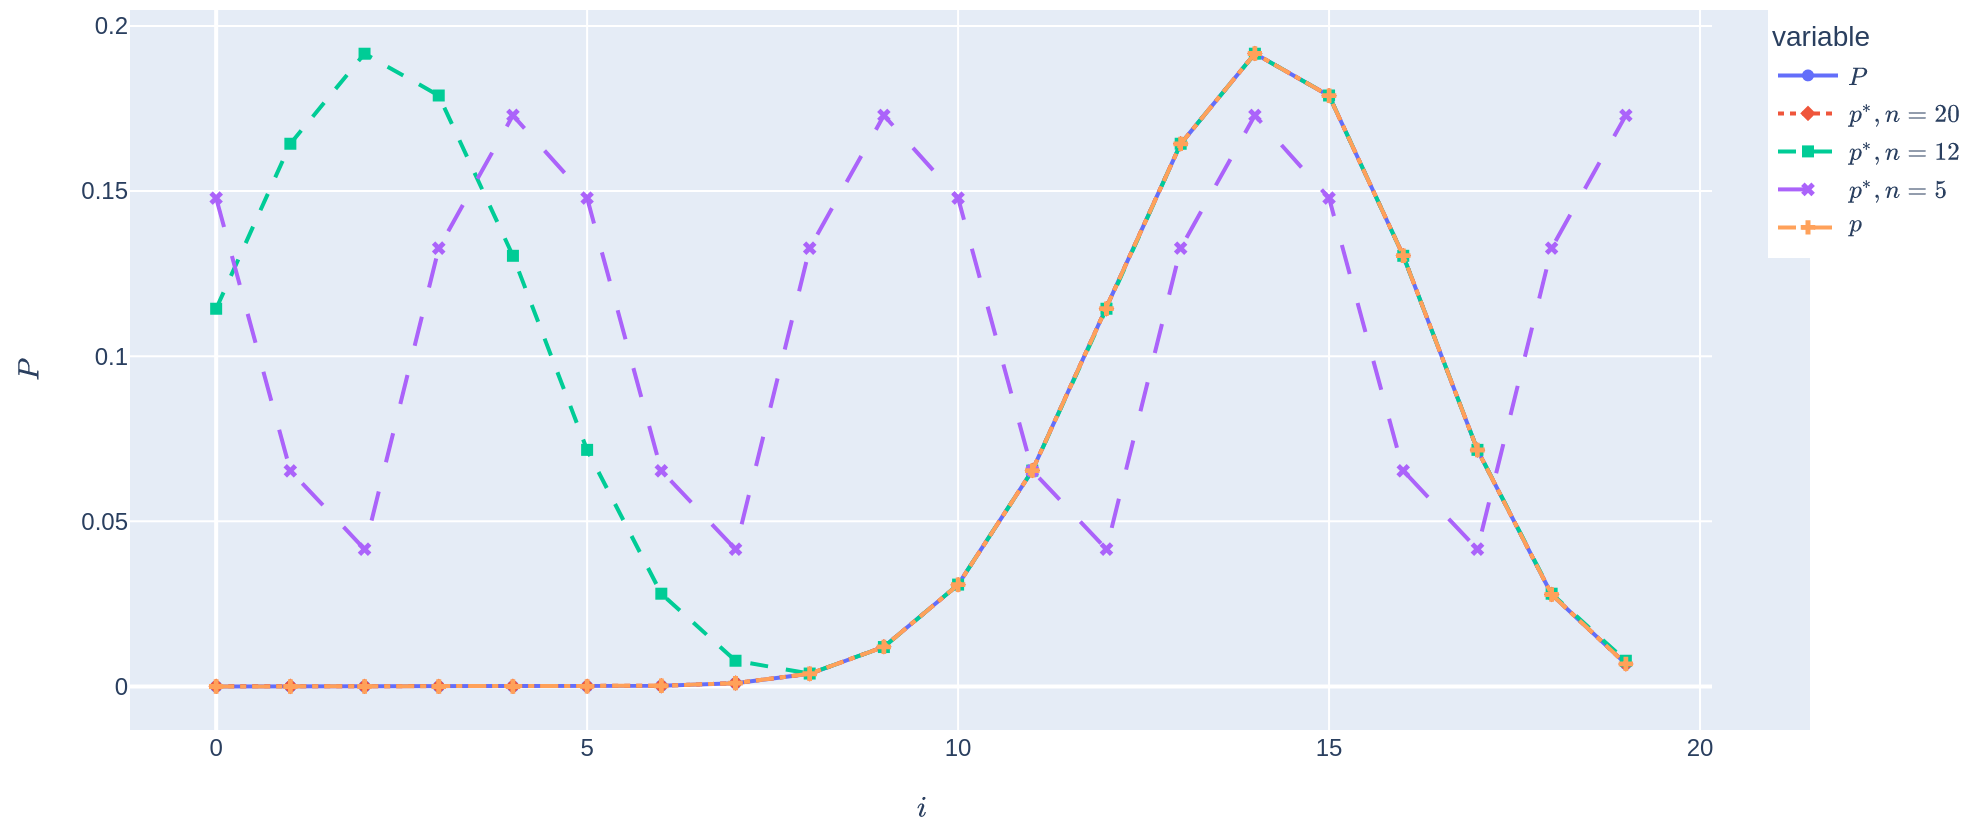
\includegraphics[height=6.8cm,width=\textwidth]{dft_figure1.png}
	\caption{Обращение характеристической функции} \label{dft_figure1}
\end{figure}

Вычисление было произведено на языке Python с заданными параметрами
\begin{equation*}
	n=20,p = 0.7,N = \{20,12\}.
\end{equation*}
Из рисунка \ref{dft_figure1} видно, что теоретическое биномиальное распределение $P$, результат обратного интегрального $p$ \eqref{int_dis_pos} и дискретного $p^*$ \eqref{dtf} преобразований совпадают при $N=20$. Однако, как показывает график, при неверном выборе шага дискретизации (в данном случае $N < n, N = 12$) распределение начинает искажаться, так как условие теоремы Котельникова \cite{ястребов2012дискретизация} не выполняется.
\subsection{Иллюстрация работы подхода на задаче теории массового обслуживания}\label{rq_3}
В данном разделе продемонстрируем эффективность предлагаемого подхода при реализации численных расчетов в задаче из \cite{blaginin2021approximation}. В данной работе получено асимптотическое приближение характеристической функции $h(u,t)$ числа обслуженных заявок в системе с повторными обращениями и вызываемыми заявками
\begin{equation}
	h(u,t)=\boldsymbol{R}e^{\boldsymbol{G}(u)t}\boldsymbol{E},
\end{equation}
которая при фиксированном $t$ является функцией только от $u$.

Здесь матрица $\boldsymbol{G}(u)$ содержит коэффициенты системы дифференциальных уравнений Колмогорова. Ее элементы выражаются через параметры модели. $\boldsymbol{R}$ --- вектор-строка, $\boldsymbol{E}$ --- единичный вектор-столбец.

Для вычисления характеристической функции необходимо вычислять матричную экспоненту $e^{\boldsymbol{G}(u)}$ , что безусловно делает задачу трудоемкой. Здесь матричную экспоненту вычисляем при помощи преобразования подобия матриц \cite{bronson1991matrix}:
\begin{equation*}
	e^{\boldsymbol{G}(u)}=\boldsymbol{T}(u)\cdot %\begin{bmatrix}
	%e^{ \Lambda_{1}(u)} & 0 &  0\\
	%0 & e^{ \Lambda_{2}(u)} & 0\\
	%0 & 0 &	e^{ \Lambda_{3}(u)}
	%\end{bmatrix}
	\boldsymbol{GJ}(u)
	\cdot \boldsymbol{T}(u)^{-1},
\end{equation*}
где $\boldsymbol{T}(u)$ --- матрица собственных векторов $\boldsymbol{G}(u)$, $\boldsymbol{GJ}(u)$ --- диагональная матрица собственных чисел $\Lambda_{n}$ матрицы $\boldsymbol{G}(u)$.

Вычисление распределения вероятностей числа обслуженных заявок в системе за некоторое фиксированное время t через интегрирование с помощью формулы \eqref{int_dis_pos} является, как уже было упомянуто, достаточно трудоемкой вычислительной задачей. Для решения этой проблемы предлагается воспользоваться формулой \eqref{dtf} ДПФ.

На рисунке \ref{dft_figure2z} видно, что результат дискретного преобразования Фурье ($p^*$) полностью совпадает с результатом вычисления при помощи интегрирования ($p$)
\begin{figure}[H]
	\centering
	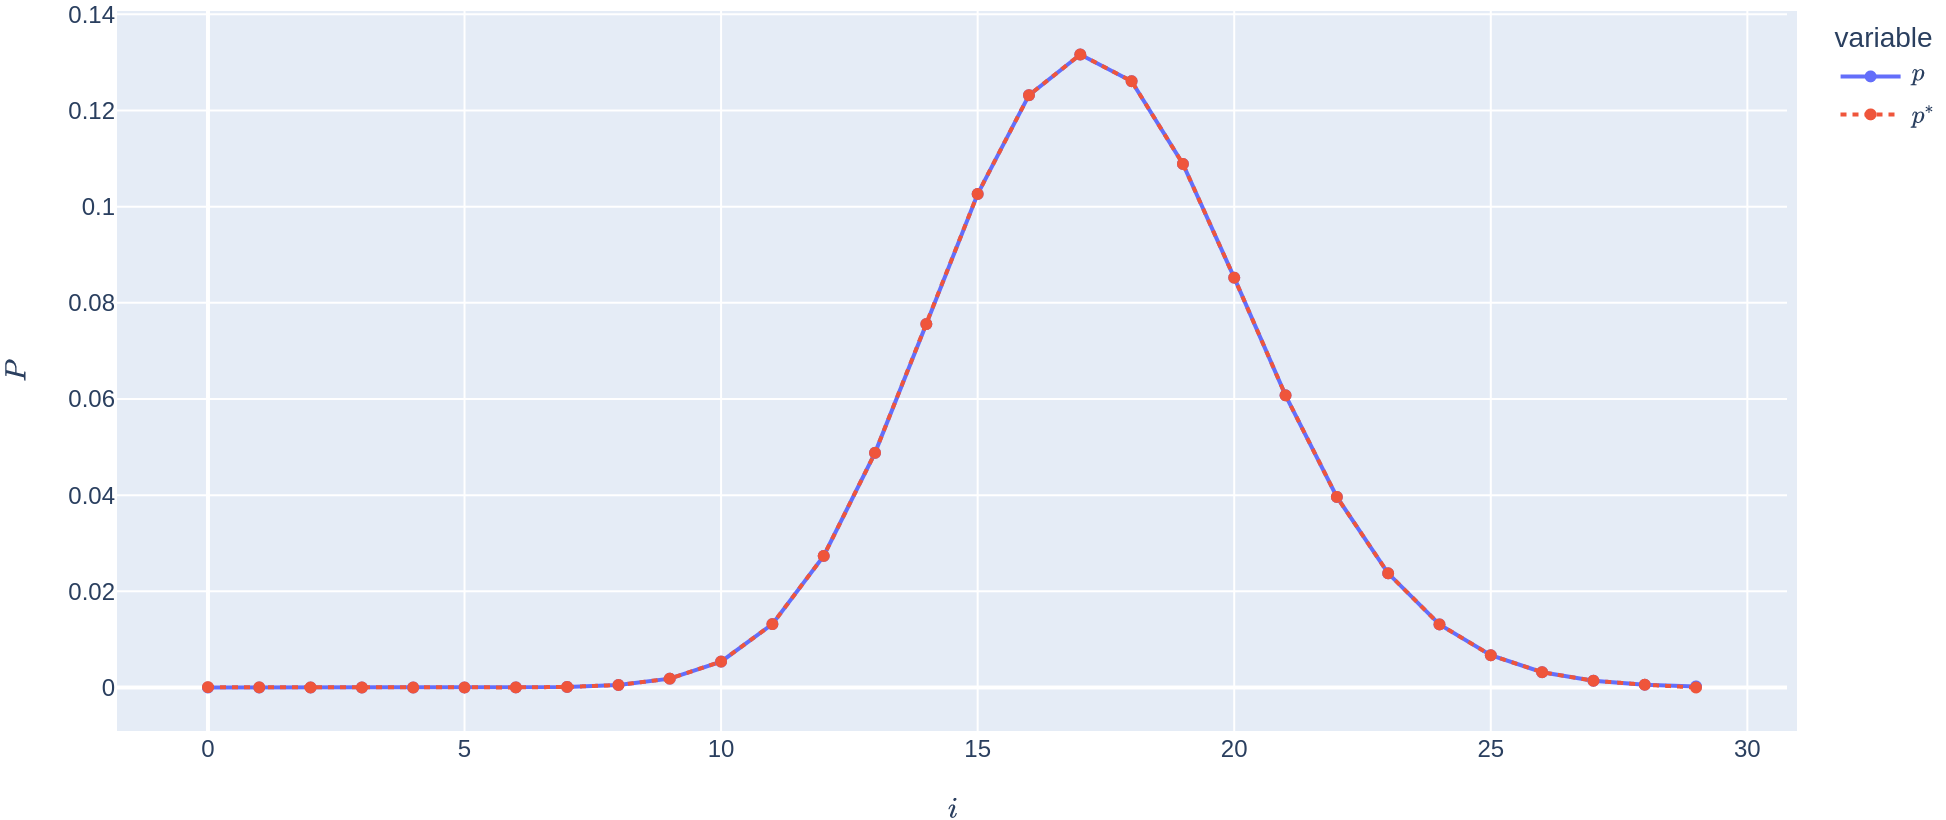
\includegraphics[scale=1,height=7cm,width=\textwidth]{dft_figure2.png}
	\caption{Сравнение распределений вероятностей, полученных с помощью интегрирования и ДПФ}
	\label{dft_figure2z}
\end{figure}

Для проверки скорости работы данного подхода к вычислению был проведен ряд тестов (400 запусков) со сравнением скорости работы алгоритмов и точности получаемого распределения при помощи расстояния Колмогорова \eqref{kdistance}.

В среднем ДПФ быстрее интегрирования более, чем в 100 раз, а среднее расстояние Колмогорова --- $4.16 \cdot 10^-6$.

Итак, предложенный метод позволяет в общем случае обращать характеристические функции гораздо более эффективно в сравнении с преобразованием Фурье, что в контексте разработанного программного комплекса позволяет быстрее вычислять асимптотические результаты и анализировать их, например, путем точечного сравнения распределений вероятности при помощи расстояния Колмогорова.

%\subsection{Вычисление коэффициента вариации MMPP}
%В данной работе одним из объектов изучения является вариация длин интервалов между моментами поступления заявок MMPP.

%Согласно \cite{вишневский2018стохастические}, вариация длин интервалов между моментами поступления заявок MMPP вычисляется как
%\begin{equation}
%	Var = \frac{\sqrt{v}}{Lg^{-1}},
%\end{equation}
%где $v$ --- дисперсия длин интервалов между моментами поступления групп запросов и рассчитывается как
%\begin{equation}
%	v = \frac{2Lg\cdot r \cdot (-D0)^{-1} \cdot E -1}{Lg^2},
%\end{equation}
%где вектор--строка $r$ --- стационарное распределение вероятностей процесса\\$\{k(t),n(t)\}$, $E$ --- единичный вектор--столбец размерности N, $Lg$ -- интенсивность %входящего потока
%\begin{equation} \label{eq_lg}
%	Lg = r\cdot \Lambda \cdot E,
%\end{equation}
%\begin{equation*}
%	D0 = Q - \Lambda - Q\cdot D,
%\end{equation*}
%где $D$ --- матрица, содержащая вероятности наступления события в потоке при смене его состояния.
\clearpage
